\documentclass[11pt,english,a4paper]{book}
\usepackage{../futhark} %I denne filen har vi alt av \usepackage, alle egendefinerte kommandoer osv.

\begin{document}

%Forside:
	\thispagestyle{empty}   %Ingen sidetall
	\forsideRapport		%Denne setter inn forsiden.
	\clearpage		%Ny side
	
%Sammendrag og forord:
	\pagestyle{plain}	%Stil på sammendrag og forord.
	\pagenumbering{roman} 	%Sidetall på formen i, ii, osv. på sammendrag, forord og innholdsfortegnelse.

	\sammendragEn{Text in abstract}
	%\coffee{4}
	\forordEn{Text in foreword}
	%\coffee{1}
	\clearpage		%Ny side

%Innholdsfortegnelse (automagisk)
	\tableofcontents
	\clearpage		%Blank side
	\thispagestyle{empty}	%Uten sidetall

%Kapitler:
	\kapittelstil %Fikser stilen i kapitlene

<<<<<<< HEAD
	\chapter{Introduction}
%In this chapter, we don't need numbering of subsections (there are none).
\setcounter{secnumdepth}{1}

\section{Problem formulation}
The problem considered in this project is the preparation of bacon in a microwave oven. Bacon is
defined as cured meat from side and back cuts of a pig. A microwave oven in this context is a
household appliance typically delivering 750 W of microwave effect at a frequency of 2.1 GHz
to a Faraday cage of volume 40 liters. 

The motivation for the problem formulation was clear. As soon as modeling of food preparation was
brought on the table, bacon seemed a prime choice. A microwave oven may seem an odd choice for
bacon, but previous experiments have shown that optimal bacon can consistently be attained with this
preparation method. Obvious advantages over traditional bacon preparation include less cleaning up
to do afterwards and a shorter time-to-plate. The caveat is that microwave preparation is less
suitable for feedback during the cooking process, as the bacon is obscured from view. To the
traditional bacon chef, used to a touch-and-go approach, this is an obstacle to implementation, as
overcooking bacon in a microwave oven yields inedible results. The
purpose of this work, then, is to establish reliable numerical simulations that can serve as a basis
for estimating cooking time for an arbitrary slice of bacon.

As the project considers the optimal preparation of bacon in a microwave oven, two natural questions
were formulated:

\begin{itemize}
  \item How is preparation of bacon in a microwave oven modelled numerically?
  \item How does water and fat content affect the preparation, and what preparation time is optimal?
\end{itemize}

\section{Reasoning behind the problem formulation}
The first question is obvious, as any attempt at predicting the preparation time necessitates a
numerical model of bacon in a microwave oven; a simple glance at the relevant
equations tells the experienced numerics person that no analytical solution
exists. With a numerical solution of the heat and mass transport equations, the
optimal preparation time can be predicted. But this presumes an understanding of
what makes good bacon. So what does?

Work done by \cite{intarwebz} and \cite{maillard} suggest that two factors are important in
determining good bacon. The first is a high enough temperature that the Maillard
reaction can take place, which happens around 140$^{circ}$C. The second is that
a significant proportion of the fat has melted and has been transported out of
the bacon. Both of these factors are naturally affected by the composition of
the bacon; especially water and fat content will play a major role.

Having identified these two factors as the important criteria for an optimal
solution, experimental work is needed to determine the correlation between
temperature and fat loss, and how finished bacon is. This is, of course, also a
subjective question - different people prefer different grades of crispness.

Another experimental question is how much of the microwave effect that is
absorbed by the bacon. The second law of thermodynamics dictates that some of
the effect is lost in the microwave magnetron, the question is how much effect
is dissipated in the bacon. This may include losses besides that of the
magnetron, which has a typical efficiency of 65\% \cite{namba}. It turns out
that common household microwave ovens are rated to include this loss,
with standardized calibration procedures published by the IEC's SC 59K, so a 750 W
microwave oven will typically draw 1.1 kW of electrical power from the mains
socket. This means using the rated power will be good enough for our purposes.

Finally, experiments are needed to verify the accuracy of the numerical results.
As heat and mass transport is a Complicated Problem, this is not guaranteed a
priori.

%Reset secnumdepth for other chapters
\setcounter{secnumdepth}{2}
 	%Kap. 1
	\chapter{The Physics}
\section{The physical system}
The physical system to be modeled is a thin, rectangular strip of bacon which is
subjected to approx. 750 watts of microwave radiation at the frequency of 2.4
GHz. To be modeled is the heat in the strip, phase transitions and transport.

\section{Our approach}
\begin{figure}[!h]
  \begin{center}
    \includegraphics[width=0.35\linewidth]{physicists.png}
  \end{center}
  \caption{Our initial approach to the problem. \url{xkcd.com/793}}
  \label{fig:xkcd_physics}
\end{figure}

Initially, our approach to modelling was to use a staggered approach: first solve the
heat equation for the three media meat, solid fat, and liquid fat, thus giving
the temperature at step $n$. Then at step $n+1$, the temperature is regarded as
known, and we solve the transport equation for liquid fat out of the bacon. Then
we know the distribution of liquid fat at step $n+2$, where we solve the heat
equations again, et cetera.

\section{The heat equations}
The differential equations governing the heat transport are all variations of the heat
equation, with various source terms, \crefrange{eq:heat1}{eq:heat3}:
\begin{align}
  \label{eq:heat1}
  (\rho c_p)_m \pd{T}{t} - \alpha_m \grad{^2 T} &= J^{MW} \quad \rm{,} \\
  \label{eq:heat2}
  \eta_s (\rho c_p)_s \pd{T}{t} - \eta_s\alpha_s \grad{^2 T} &= J^{MW} - J^{Melt}  \quad \rm{,} \\
  \label{eq:heat3}
  \eta_l (\rho c_p)_l \pd{T}{t} - \eta_s\alpha_l \grad{^2 T} - \eta_l(\rho c_p)_l(\v{v}\cdot
  \grad{})T &= J^{MW}  \quad \rm{.}
\end{align}
Here the subscript $m$ denotes meat, $s$ denotes solid fat, and $l$ denotes
liquid fat. $J^{MW}$ is the source term representing the microwave oven.
Here this is modelled as a cylindrically symmetric term,
with the radial power distribution on the form \cref{eq:effektfordeling},
\begin{equation}
  J^{MW}(r) = 0.5 + 2.55008x - 0.588013x^2 + 0.032445x^3 + 0.00124411x^4 - 0.0000973516x^5 \rm{,}
  \label{eq:effektfordeling}
\end{equation}
i.e. a fifth degree polynomial, interpolated from the results in
\cite{huang+zhu}. This is an effective source term, and is considered valid for
cooking times that are large compared to the rotation period of the plate inside
the microwave oven. This term may look confusing, so it has been illustrated in
\cref{fig:microwave}.\\

\begin{figure}[h!]
  \begin{center}
    \includegraphics[width=0.7\textwidth]{microwave.pdf}
  \end{center}
  \caption{The microwave effect distribution}
  \label{fig:microwave}
\end{figure}

Furthermore, there is the term $J^{Melt}$ which represents heat loss due to
latent heat absorbed in the solid-liquid phase transition. This can be written as 
\[ \frac{L \rho}{T_2-T_1} \pd{T}{t} \rm{,} \quad T \in (T_1,T_2) \rm{,}\]
with $L$ the latent heat of the fat, and where the fat is melting between the temperatures 
$T_1$ and $T_2$. For fat these are typically around 30-50$^\circ$C. For $T \notin (T1,T2)$ 
this term is zero, and it is readily seen that this is equivalent to a modification of the constant
$c_{p,l}$ in \cref{eq:heat2} when $T \in (T1,T2)$, thus it is not a serious
complication.\\

In the last of the heat equations, there also appears what is called a
convective derivative, on the form $(\v{v}\cdot \grad{})T$. This is a somewhat
more complicated term, and is essentially a modification due to transport of
liquid fat implying a transport of heat. But we're in luck! \\

As the bacon strip is essentially two-dimensional, transport will almost
exclusively happen in the vertical (small) direction, and also the
source terms don't vary in the vertical direction. As this term will be a transport
of heat in the vertical direction, it will not affect the heat transport in
the horisontal directions.  As we're not really
interested in the vertical temperature distribution, this means that we can
happily neglect this term, in the spirit of Richard Feynmann: ``it doesn't give
any new physics''.

\section{The transport equations}
The transport equation used in our approach is the one-dimensional Navier Stokes
equation, with the additional assumptions of an incompressible, Newtonian flow.
This is the same as ignoring phenomena where sound waves or shock waves are
important, which makes sense here. This leads to \cref{eq:navier-stokes}
\begin{equation}
  \rho \left(\pd{v}{t} + v \cdot \pd{v}{x}\right) = -\pd{p}{x} + \mu \nabla^2 v + f
 \label{eq:navier-stokes}
\end{equation}
where $f$ includes any additional forces, such as gravity. An interesting term here is $\pd{p}{x}$, where
$p$ is the pressure in the fluid. Following the work by \cite{brent}, we replace
this with a term inspired by \cref{carman-kozeny}
\begin{equation}
  \pd{p}{x} = -C\frac{ (1-\epsilon)^2}{\epsilon^3} v_a
  \label{carman-kozeny}
\end{equation}
where $\epsilon = \epsilon(z)$ is the melted fraction in the current volume element, and
$v_a$ is an apparent velocity. As the volume element melts, $\epsilon$ goes from
zero to one, and $\pd{p}{x}$ goes from a very large value to zero. This is known 
as the Carman-Kozeny equation for flow in a pouros medium, and is applicable to 
materials where melting does not happen at one specific temperature, but instead 
over a range of temperatures (non-isothermal phase change). \cite{poirier} \\

This melting behavior is typical for a material with a combination of slightly different
fats, e.g. chocolate or in this case bacon. When a volume element is partially
melted, it is assumed to have a dendritic structure, and it is said to be in a
``mushy'' phase. The dendritic structure itself, and whether the flow is parallell or
orthogonal to the dendritic structure, will influence the constant C. \\

Using the procedure outlined in \cite{poirier}, the constant $C$ was estimated to be
$8 \times 10^8$, where flow is assumed to be parallell to the dendritic
structure, and the primary dendritic arm distance in bacon fat was measured to be
about 2.5 mm. The assumption of parallell flow dictates the value of the Kozeny
constant yielding the final value for $C$.\\

Influenced by these considerations, the term $\pd{p}{x}$ in
\cref{eq:navier-stokes} was replaced by \cref{eq:pressure}
\begin{equation}
  \pd{p}{x} =  -C\frac{ (1-\epsilon)^2}{(\epsilon+d)^3} v
  \label{eq:pressure}
\end{equation}
where $d$ is a tiny constant introduced simply to avoid dividing by zero in the
numerical procedure.\\

Introducing this term has two effects. First of all, for a solid element,
$\pd{p}{x}$ becomes very large, and forces the velocity to be zero. When the
element starts melting, the flow will mimic the Carman-Kozeny flow, which is
realistic for a porous medium, and finally in the molten stage, the ordinary
pressureless Navier Stokes equations are recovered.\\

Alas, the numerical implementation of the transport equation was not completed
within the timeframe of the project. The theory is still presented here for
completeness.

An alternative route suggested at the last moment is to take the pressureless
Navier Stokes equation, i.e. $\pd{p}{x} = 0 \forall x,t$, and add a source term
proportional to $\pd{\epsilon}{t}$. To understand this, it helps to think of the
Navier Stokes equation as a diffusion equation in momentum, with an extra
convective derivative. With an initial condition of zero flow everywhere, and
absorbing boundary conditions 

		%Kap. 2
	\chapter{Numerics}

\section{Numerical schemes for the heat equation}

The heat equation is on the form
\begin{equation}
\frac{\partial u}{\partial t}=\mu \grad{^2 u} + K,
\label{heatequation}
\end{equation}
Here K is a constant, and we thus neglect it in the discretization of (\ref{heatequation}).\\

In this project the Cranch-Nicholson method was used to discretize the heat
equation \cref{eq:heat1} in 3D over a finite grid. This method was chosen because
it is unconditionally stable, and it converges in second order in time and
space, as is shown below. \\

The Crank-Nicholson method is based on the equation \cref{integral}, where the trapezoidal rule \cref{trapezoidalrule} is used to approximate the integral on the right hand side. We insert the right hand side of the heat equation in the resulting expression \cref{res}, and use Taylor-expansion to obtain the discretizaion. We use the notation \cref{notations} in the rest of this document.

\begin{equation}
\partial_{x}^{k}u=\frac{\partial^{k}u}{\partial^{}x^{k}},\quad \quad \partial_{t}^{k}u=\frac{\partial^{k}u}{\partial^{}t^{k}} \quad \quad u_{m}^{n+\alpha k } = u(x_{m},t_{n}+\alpha k)
\label{notations}
\end{equation}

\begin{equation}
u(x_m,t_{n+1}) - u(x_m,t_n) = \int_{t_n} ^{t_{n+1}} u_t(x_m,t) dt
\label{integral}
\end{equation}

\begin{equation}
\int_0^k f(t) dt = \frac{1}{2} k (f(0) - f(k)) -\frac{1}{12} k^3 f''(\frac{k}{2}) + ...
\label{trapezoidalrule}
\end{equation}
We thus obtain
\begin{eqnarray}
\label{res}
u_m^ {n+1} &=& u_m^ n + \frac{1}{2} k(\partial_t u_m^n + \partial_t u_m^{n+1}) - \frac{1}{12} k^3 \partial_t ^3 u_m^{n+\frac{1}{2}} + ...\\
&\stackrel{\text{\tiny heat eq.}}{=}& u_m^ n + \frac{1}{2} \mu k(\partial_x^2 u_m^n + \partial_y^2 u_m^n + \partial_z^2 u_m^n + \partial_x^2 u_m^{n+1} + \partial_y^2 u_m^{n+1} + \partial_z^2 u_m^{n+1}) - \frac{1}{12} k^3 \partial_t ^3    u_m^{n+\frac{1}{2}} + ... \nonumber
\end{eqnarray}
Using central differences \cref{centraldiff}, and denoting the step sizes in $x, y, z$ direction by $h, f, g$ respectively gives
\begin{eqnarray*}
u_m^{n+1} &=& u_m^ n + \frac{1}{2} \mu k(\frac{1}{h^2}\delta_x^2 u_m^n + \frac{1}{f^2}\delta_y^2 u_m^n + \frac{1}{g^2}\delta_z^2 u_m^n + \frac{1}{h^2}\delta_x^2 u_m^{n+1} + \frac{1}{f^2}\delta_y^2 u_m^{n+1} + \frac{1}{g^2}\delta_z^2 u_m^{n+1}) \\
  &&- \frac{1}{2} \mu k (\frac{1}{12}h^2\partial_x^4 u_m^n +
  \frac{1}{12}g^2\partial_y^4 u_m^n + \frac{1}{12}f^2\partial_z^4 u_m^n +
  \frac{1}{12}h^2\partial_x^4 u_m^{n+1} + \frac{1}{12}g^2\partial_y^4
  u_m^{n+1}\\
  &&+ \frac{1}{12}f^2\partial_z^4 u_m^{n+1} + \cdots)
  - \frac{1}{12} k^3 \partial_t ^3 u_m^{n+\frac{1}{2}} \\ 
  %&=& u_m^n + \frac{r}{2}(\delta_x^2 u_m^n + \delta_x^2 u_m^{n+1}) + \frac{p}{2}(\delta_y^2 u_m^n + \delta_y^2 u_m^{n+1}) + \frac{q}{2}(\delta_z^2 u_m^n + \delta_z^2 u_m^{n+1}) + \tau_m^n
\end{eqnarray*}
where
\begin{equation}
\delta_{r}^{2}U_m^{n}=\frac{U_{m+1}^{n}-2U_m^{n}+U_{m-1}^{n}}{{\Delta r}^{2}}
\label{centraldiff}
\end{equation}
At this point it may be instructive to use \cref{fig:stencil-numerics} as a guideline.

\begin{figure}[h!]
  \begin{center}
    \includegraphics[width=0.7\textwidth]{stencil.png}
  \end{center}
  \caption{Stencil for the Crank Nicolson method}
  \label{fig:stencil-numerics}
\end{figure}

We thus obtain the implicit method for the heat equation
\begin{equation}
u_m^{n+1}-\mu k(\frac{1}{h^2}\delta_x^2 u_m^{n+1}-\frac{1}{f^2}\delta_y^2 u_m^{n+1}-\frac{1}{g^2}\delta_z^2 u_m^{n+1})=u_m^n + \mu k(\frac{1}{h^2}\delta_x^2 u_m^n + \frac{1}{f^2}\delta_y^2 u_m^n +\frac{1}{g^2}\delta_z^2 u_m^n)
\label{crank}
\end{equation}
with truncation error error
\begin{eqnarray}
\frac{\tau_m^ n}{k} &=& -\frac{1}{12} \mu k^2 \partial_t^2 u_m^{n+\frac{1}{2}} - \frac{1}{12} \mu h^2 \partial_x^4 u_m^{n+\frac{1}{2}} - \frac{1}{12} \mu g^2 \partial_y^4 u_m^{n+\frac{1}{2}} - \frac{1}{12} \mu f^2 \partial_z^4 u_m^{n+\frac{1}{2}}\\
&=& \mathcal{O} (k^2 + h^2 + g^2 + f^2)
\label{truncerror}
\end{eqnarray}

Here we have used that $\frac{1}{2}(\partial_x^4 u_m^n + \partial_x^4 u_m^{n+1}) = \partial_x^4 u_m^{n+\frac{1}{2}} + \mathcal{O} (k^2)$. 
The truncation error $\tau_m^n \Rightarrow 0$ as $h,f,g,k \Rightarrow 0$, and the Crank-Nicholson method is consistent for the heat equation. To see if the method converges we perform a von Neumann analysis of the numerical scheme.

\section{Von Neumann analysis of the Crank-Nicholson-scheme}

The von Neumann analysis is based on Fourier analysis, see \cite{aarseth}. The method consist of substituting 
\begin{equation*}
	U_m^n=\xi^n e^{i \beta x_m} \quad \quad  i=\sqrt{-1}
\end{equation*}
in the difference equation and solving for $\xi$.
For the method to be stable it has to meet the condition
\begin{equation}
	\mid{\xi}\mid \leq 1
	\label{stabcond}
\end{equation}

Here we only perform the von Neumann analysis for the one-dimensional heat
equation, giving the expression
\begin{equation*}
\xi^{n+1} e^{i\beta x_{j}} = \xi^{n} e^{i\beta x_j}\left(1-2D\right) + \xi^{n+1}D\left(e^{i\beta x_{j+1}} - 2e^{i\beta  x} + e^{i\beta x_{j-1}}\right) + \xi^{nD}\left(e^{i\beta x_{j+1}} + e^{i\beta x_{j-1}}\right)
\end{equation*}

where
\begin{equation*}
D = \frac{1}{2}\frac{\alpha\Delta t}{(\Delta x)^2}
\label{eq:crank-D}
\end{equation*}

Dividing  by $\xi^ne^{i\beta x_j}$, and using $x_{j+1} = x_j + h$ one obtains    %\href{eq:crank-D}
\begin{eqnarray*}
\xi\left[1-D\left(2\cos{\beta h} - 2\right)\right] &=& 1 - 2D\left(1-\cos{\beta h}\right) \\
\cos{\beta h} &=& 1-2\sin^2{\frac{\beta h}{2}} \\
\xi\left(1+4D\sin^{2}{\frac{\beta h}{2}}\right) &=& 1 - 4D\sin^2{\frac{\beta h}{2}} \\
\xi &=& \frac{1-4D\sin^2{\frac{\beta h}{2}}}{1+4D\sin^2{\frac{\beta h}{2}}}
\end{eqnarray*}
As the maximum value of $\sin^2{x}$ is 1, the methods meets the stability condition \ref{stabcond}.
\begin{equation}
|\xi | = \left|\frac{1-4D}{1+4D}\right|
\end{equation}

Since D is always positive, we get that the Crank-Nicolson
scheme for the heat equation is \emph{unconditionally stable}. In practice it
may happen that the method oscillates if the time steps and space steps do not
fulfill a CFL-condition\footnote{Courant-Friedrichs-Levy condition}.
\\
\\
From Lax' equivalent theorem, which states that a consistent difference scheme will converge if and only if it is stable, the Crank-Nicholson scheme will converge.


%\section{Truncation error in the Crank-Nicolson scheme}

%The Crank-Nicholson method is based on the trapezoidal rule. From the trapezoidal rule the truncation error is represented by
%\begin{equation*}
%\int_0^k f(t) dt = \frac{1}{2} k (f(0) - f(k)) -\frac{1}{12} k^3 f''(\frac{k}{2}) + ...
%\end{equation*}
%Using the formula
%\begin{equation*}
%	u(x_m,t_{n+1}) - u(x_m,t_n) = \int_{t_n} ^{t_{n+1}} u_t(x_m,t) dt
%\end{equation*}
%and approximating the integral by the trapezoidal rule, and abbreviate the notation $u_m^{n+1/2} = u(x_m,t_n+\frac{1}{2} k)$, one obtain
%\begin{eqnarray*}
%u_m^ {n+1} &=& u_m^ n + \frac{1}{2} k(\partial_t u_m^n + \partial_t u_m^{n+1}) - \frac{1}{2} k^3 \partial_t ^3 u_m^{n+\frac{1}{2}} \\
%		   &\stackrel{\text{\tiny heat eq.}}{=}&  u_m^ n + \frac{1}{2} k(\partial_x^2 u_m^n + \partial_y^2 u_m^n + \partial_z^2 u_m^n + \partial_x^2 u_m^{n+1} + \partial_y^2 u_m^{n+1} + \partial_z^2 u_m^{n+1}) - \frac{1}{2} k^3 \partial_t ^3 u_m^{n+\frac{1}{2}}
%\end{eqnarray*}
%Discretizing the double derivative with central differences, and denoting the step sizes in $x, y, z$ direction by $h, f, g$ respectively, gives
%\begin{eqnarray*}
%u_m^{n+1} &=&  u_m^ n + \frac{1}{2} k(\frac{1}{h^2}\delta_x^2 u_m^n + \frac{1}{f^2}\delta_y^2 u_m^n + \frac{1}{g^2}\delta_z^2 u_m^n + \frac{1}{h^2}\delta_x^2 u_m^{n+1} + \frac{1}{f^2}\delta_y^2 u_m^{n+1} + \frac{1}{g^2}\delta_z^2 u_m^{n+1}) \\
% 		  &&- \frac{1}{2} k (\frac{1}{12}h^2\partial_x^4 u_m^n + \frac{1}{12}g^2\partial_y^4 u_m^n \frac{1}{12}f^2\partial_z^4 u_m^n + \frac{1}{12}h^2\partial_x^4 u_m^{n+1} + \frac{1}{12}g^2\partial_y^4 u_m^{n+1} \frac{1}{12}f^2\partial_z^4 u_m^{n+1} ) \\
% 		  &&- \frac{1}{2} k^3 \partial_t ^3 u_m^{n+\frac{1}{2}} \\
% 		  &=& u_m^n + \frac{r}{2}(\delta_x^2 u_m^n + \delta_x^2 u_m^{n+1}) + \frac{p}{2}(\delta_y^2 u_m^n + \delta_y^2 u_m^{n+1}) + \frac{q}{2}(\delta_z^2 u_m^n + \delta_z^2 u_m^{n+1}) + \tau_m^n
%\end{eqnarray*}
%where $r = k/h^2$, $p = k/f^2$, $q = k/g^2$, and $\tau_m^n$ is the truncation error times $k$. The expression for $\tau_m^n$ is
%\begin{equation*}
%\tau_m^n = -\frac{1}{12} k^3 \partial_t^2 u_m^{n+\frac{1}{2}} - \frac{1}{12} k h^2 \partial_x^4 u_m^{n+\frac{1}{2}} - \frac{1}{12} k g^2 \partial_y^4 u_m^{n+\frac{1}{2}} - \frac{1}{12} k f^2 \partial_z^4 u_m^{n+\frac{1}{2}}
%\end{equation*}
%where we have used $\frac{1}{2}(\partial_x^4 u_m^n + \partial_x^4 u_m^{n+}) = \partial_x^4 u_m^{n+\frac{1}{2}} + O(k^2)$. Hence, the truncation error is 
%\begin{eqnarray*}
%\frac{\tau_m^ n}{k} &=& -\frac{1}{12} k^2 \partial_t^2 u_m^{n+\frac{1}{2}} - \frac{1}{12} h^2 \partial_x^4 u_m^{n+\frac{1}{2}} - \frac{1}{12} g^2 \partial_y^4 u_m^{n+\frac{1}{2}} - \frac{1}{12} f^2 \partial_z^4 u_m^{n+\frac{1}{2}}\\
%					&=& O(k^2 + h^2 + g^2 + f^2)
%\end{eqnarray*}

	%Kap. 3
	
\chapter{Implementation}

\section{Tools}

The programming language chosen to implemented the system was c++.
The arguments leading to this choice was:

\begin{itemize}
\item Most of the group members had some earlier experience with the language.
\item It allows for a high level of abstraction without loosing control of the
underlying hardware.
\item The code can be easily parallelized for shared memory machines using OpenMP.
\item Many libraries exist for c++ that implements highly optimized linear algebra
functionality.
\end{itemize}

Other languages cosidered where Matlab and c.

The tool chosen to visualize the resulting data was gnuplot and ffmpeg. Writing a
program using OpenGL was considered, but dismissed on the grounds of beeing too time consuming.

\section{Program design}

\begin{figure}[!h]
  \begin{center}
    \includegraphics[width=0.5\linewidth]{classdiagram.png}
  \end{center}
  \caption{Class diagram of c++ implementation}
  \label{fig:class_diagram}
\end{figure}

The program mainly consist of three parts:

\begin{itemize}
\item C++ implementation of Linear algebra functionality of the discrete equations.
\item C++ implementation of the conjugate gradient method for solving the
equations described.
\item Bash script for generating plots and and movie of the generated data.
\end{itemize}

See \cref{fig:class\_diagram} for a class diagram of c++ implementation.

The Bash script is not discussed in further detail as it can be considered to be
very simple.

\section{The physical system}

The main task of the physical system is to implement a matrix-vector multiplication
procedure for the heat equation to be used in the conjugate gradient method, 
a method for calculating the heating properties of the microwave and a method 
for calculating the velocity of mass transfer.

\subsection{Partitioning of the problem}

The problem is to perform the multiplication of a sparse, symmetrix, matrix with a
vector. To describe this procedure we have vectors $a$, $b$ and $t$ containing alpha,
beta, and temperature values respectively. The alpha values represent the heat 
conduction properties, the beta values describe the substance's ability to heated
by microwaves and the temperature values naturally contains the temperatures.

\begin{figure}[!h]
  \begin{center}
    \includegraphics[width=0.5\linewidth]{grid.png}
  \end{center}
  \caption{Grid}
  \label{fig:grid}
\end{figure}

We say that position $j$ of the vectors is given by:
\begin{equation}
j = z*n_x*n_y + y*n_x + x
\end{equation}

where $n_x$, $n_y$, $n_z$ is the number of points in the $x$, $y$ and $z$ directions
respectively. See \cref{fig:grid}

The center of the stencil, given by $j$ can be described by the equations:
\begin{equation}
x = j \% n_x \\
y = ( j // nx ) \% ny
z = ( j // nx // ny )
\end{equation}

where $//$ and $\%$ is the integer division and modulo operators respectively.

In addition to this, we define two more vectors and one more matrix:

\begin{figure}[!h]
  \begin{center}
    \includegraphics[width=0.5\linewidth]{stencil.png}
  \end{center}
  \caption{Stencil}
  \label{fig:stencil}
\end{figure}

The offset matrix represents the neighbours in the stencil (see \cref{fig:stencil}:
\begin{equation}
\[
O =
\left[
\begin{array}{ccc}
0 & 0 & -1 \\
0 & -1 & 0 \\
-1 & 0 & 0 \\
0 & 0 & 0 \\
1 & 0 & 0 \\
0 & 1 & 0 \\
0 & 0 & 1 \\
\end{array}
\right]
\]
\end{equation}

The delta vector representing the difference in time and distance used in the heat
equation:
\begin{equation}
D = \{ \frac{dt}{dz^2}, \frac{dt}{dy^2}, \frac{dt}{dx^2}, 0, \frac{dt}{dx^2}, \frac{dt}{dy^2}, \frac{dt}{dz^2} \}
\end{equation}

The matrix containing the offsets relative to the diagonal in the matrix we are multiplying
with:
\begin{equation}
R = \{ -n_x*n_y, -n_x, -1, 0, 1, n_x, n_x*ny \}
\end{equation}

This is all the information we need to perform the necessary operations.

\subsection{Updating alpha and beta values}

When updating the alpha and beta values, we simply loop through the temperature
vector, and update the alpha and beta vectors to their correct values using the
physical contants describing the substance at that point.

\subsection{Calculating the distribution of the microwave effect}

This is done according to \cref{eq:effektfordeling} and by multiplying the
resulting distribution by the microwave effect and dividing by the volume at each point
in the grid.

\subsection{The matrix-vector multiplication procedure}

The matrix-vector multiplication procedure takes advantage of the fact that our 
matrix is sparse and that our problem is well defined. Thus, the algorithm used
will complete in $m$ iterations where $m$ is the number of non-zero entries in 
the matrix. $m$ is approximately equal to $7m$.

\section{The conjugate gradient method as an iterative algorithm}

The method (conjugate gradient) used to solve the system of equations is based on 
the steepest descent algorithm, however, it results in the exact solution within
$n$ iterations. This is, however, assuming we have infinite floating point accuracy.

The iterative conjugate gradient method lets us define an acceptable error, and stops
once our solution has an error below what is acceptable.

In our implementation, we recompute the correct residual to avoid accumulation of
floating point precision errors, however, this is not done at each iteration, and may
result in the need of more than $n$ iterations for the algorithm to complete.

\section{The main procedure}

\begin{itemize}

  \item Initialize problem; define grid-size, dimensions of bacon, partitioning of fat vs meat
  and internal and external temperature.
  \item Allocate necessary memory
  \item Initialize physical system
  \item Initialize internal temperature
  \item Initialize internal flow
  \item Calculate boundary conditions
  \item Calculate micro-wave field
  \item Initialize conjugate gradient solver
  \item loop
  \begin{itemize}
    \item Update alpha and beta values
    \item Calculate diagonal
    \item Set signs for right side multiplication (t=n)
    \item Multiply right side of heat equation
    \item Add micro-wave effect to right side of equation
    \item Set signs for left side of equation (t=n+1)
    \item Solve using conjugate gradient method
  \end{itemize}

\item Deallocate memory
\end{itemize}

 %Kap. 4
	\chapter{Experiments}
\section{Equipment}
\begin{itemize}
\item 750W Microwave oven
\item Bacon: two types, thick bacon (``skogsbacon'') and regular bacon.
\item Ruler
\item Slide caliper
\item Mettler AE50 (weight)
\item Paper
\item Grease-proof paper
\item Scissors
\end{itemize}

\section{Execution}

The baocn slice was laid between one sheet of paper on top, and one sheet of
grease-proof paper beneath. Earlier experiments with dual layer paper had
resulted in fusing of the bacon and paper. Still we needed to absorb the fat
output, so a compromise was to combine paper (for fat absorption) and
grease-proof paper (preventing fat spillage). $\\$

First we measured the weight of the wrapping (paper and grease-proof paper), and
then we measured the dimensions of the bacon; weight, length, thickness and
width. The bacon slice was wrapped and baked in the microwave oven for the
desired amount of time. After completion we measured new dimensions, both of
bacon and wrapping and assigned a number between 0.0-1.0 describing how crisp
the bacon had gotten.

\section{Measurements}

First we measured weight gain in the wrapping, then weight loss in the bacon. We
assumed that all gain in the wrapping came from fat absorption, and that the
weight loss in the bacon consisted of fat melting and water evaporation. The new
dimensions of the bacon were also documented. $\\$

The assumptions combined with our measurements made it possible to quantify fat
loss, water loss and shrinkage of the bacon. This gave us the plots in
\cref{fig:thick_bacon} and \cref{fig:regular_bacon}.

\begin{figure}[ht!]
\subfloat[Thick
bacon]{\label{fig:thick_bacon}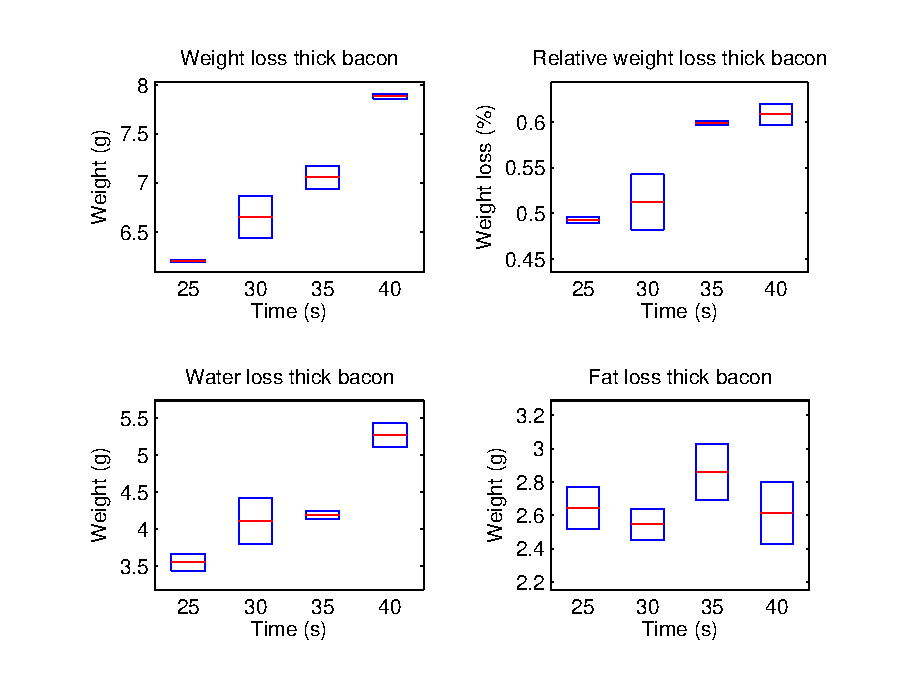
\includegraphics[width=0.5\textwidth]{thick_bacon}}\qquad
\subfloat[Regular bacon]{\label{fig:regular_bacon}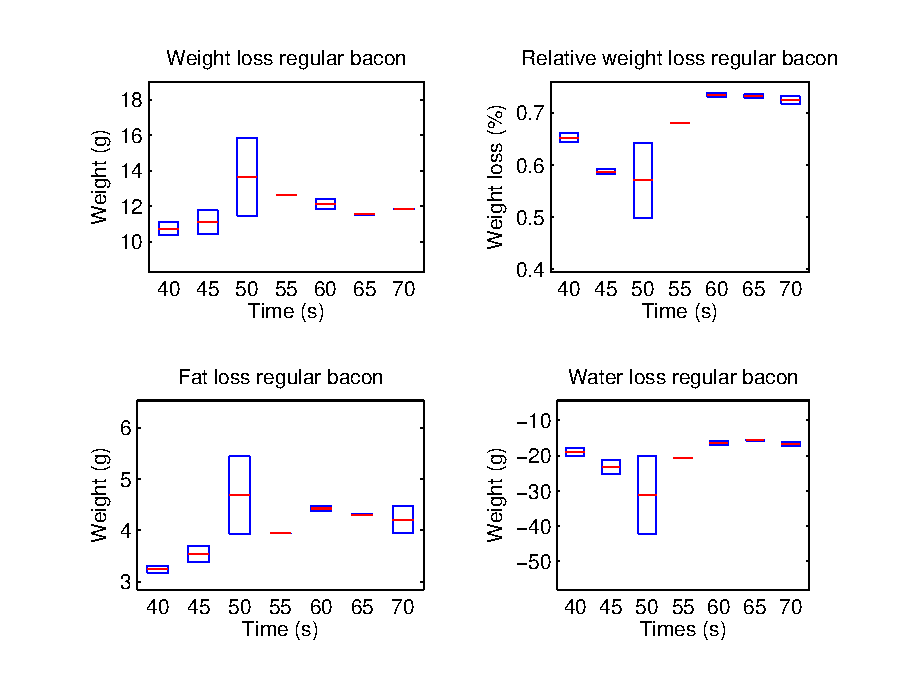
\includegraphics[width=0.5\textwidth]{regular_bacon}}
\caption{Schematic representation of measured data}
\label{fig:baconplot}
\end{figure}

\section{Results and discussion}

As we can see in \cref{fig:thick_bacon} the water loss from 30-35 seconds is
approximately constant, the fat loss on the other hand is increasing on the same
time interval. This shows that around 30-35 seconds fat starts to melt,
``stealing'' heat from the water, this is in correspondence with weight loss as
a function of time. The fat loss continues to be linearly
increasing up to about 50 seconds, see \cref{fig:regular_bacon}. After 50
seconds the fat loss stabilizes, indicating that no more fat can be lost, and
that further baking time results in burnt bacon. $\\$

These results coincides with our anticipations, that the weight loss would
stabilize after a critical time. Something that is clearly demonstrated in
\cref{fig:baconplot}. It is worth commenting that the big variation in
\cref{fig:regular_bacon} for $t = 50$s is due to one enormous (relative to the
others) bacon slice.
 %Kap. 5
	\include{resultats_numerics} %Kap. 6
	\chapter{Conclusion}
\section{Discussion of the results}

\section{Conclusion}
The performed numerical simulations and experiments with bacon preparation
in a microwave oven gave satisfactory results so far as they were implemented. 
The numerical simulations of the heat equations gave reasonable results in agreement
with experiments. An implementation of the transport equation would have been
more satisfactory, and is suggested as a possibility for future work in this
direction. The experiments performed suggest that the fat transport is
complicated, and that gravity is not dominating the flow. 


	%Kap. 7
=======
	\chapter{Innledning}
\section{Innledning}
Her skal innledningen stå. Pass på å sitere \cite{schwarz}.
 	%Kap. 1
	\chapter{Teori}
\section{Gruppeteori}
\lipsum{3-5}
\section{Kommunikasjonsteori}
\lipsum{6-8}
		%Kap. 2
	\chapter{Numerikk}
\section{Numerikk}
\lipsum[1-3]
	%Kap. 3
	\chapter{Implementation}

\section{Tools}

The programming language chosen to implemented the system was c++.
The arguments leading to this choice was:

\begin{itemize}
\item Most of the group members had some earlier experience with the language.
\item It allows for a high level of abstraction without loosing control of the
underlying hardware.
\item The code can be easily parallelized for shared memory machines using OpenMP.
\item Many libraries exist for c++ that implements highly optimized linear algebra
functionality.
\end{itemize}

Other languages cosidered where Matlab and c.

The tool chosen to visualize the resulting data was gnuplot and ffmpeg. Writing a
program using OpenGL was considered, but dismissed on the grounds of beeing too time consuming.

\section{Program design}

The program mainly consist of three parts:

\begin{itemize}
\item C++ implementation of Linear algebra functionality of the discrete equations.
\item C++ implementation of the conjugate gradient method for solving the
equations described.
\item Bash script for generating plots and and movie of the generated data.
\end{itemize}

The Bash script is not discussed in further detail as it can be considered simple.

\section{The physical system}

The main task of the physical system is to implement a matrix-vector multiplication
procedure for the heat equation and a method of calculating the heating properties of
a microwave.

\subsection{Partitioning of the problem}

\subsection{Updating alpha and beta values}

\subsection{Calculating the distribution of the microwave effect}

\subsection{The matrix-vector multiplication procedure}

\section{The conjugate gradient method as an iterative algorithm}


 %Kap. 4
	\chapter{Eksperimenter}
\section{Eksperimenter}
\lipsum[1-3]
 %Kap. 5
	\chapter{Numerikkresultater}
\section{Numerikkresultater}
\lipsum[1-3]
 %Kap. 6
	\chapter{Konklusjon}
\section{Konklusjon}
\lipsum[1-3]
	%Kap. 7
>>>>>>> 7058789ac84f4f187b361c86910142d6ef70d782

%Referanser:
	\bibliographystyle{plain}
	\bibliography{references.bib}

\end{document}

